\documentclass{standalone}
\usepackage{tikz}
\usepackage{ctex,siunitx}
\setCJKmainfont{Noto Serif CJK SC}
\usepackage{tkz-euclide}
\usepackage{amsmath}
\usetikzlibrary{patterns, calc}
\usetikzlibrary {decorations.pathmorphing, decorations.pathreplacing, decorations.shapes,}
\begin{document}
\small
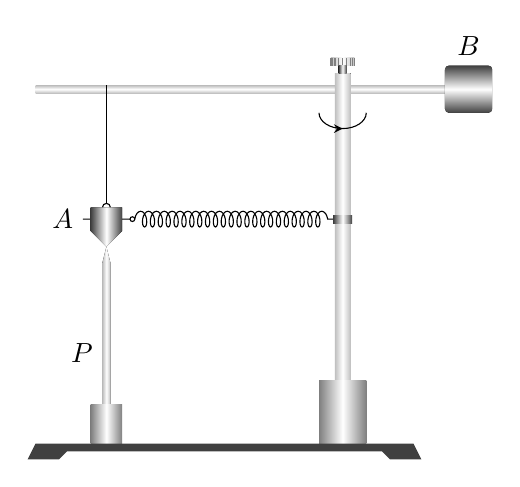
\begin{tikzpicture}[>=latex,scale=1]
  \fill[top color=lightgray,bottom color=lightgray,middle color=white](-3.9,4.45)rectangle(1.3,4.55);
  \fill[top color=darkgray,bottom color=darkgray,middle color=white,rounded corners=0.5mm](1.9,4.2)rectangle(1.3,4.8);
  \node at(1.6,4.8)[above]{$B$};
  \fill[left color=lightgray,right color=lightgray,middle color=white](-0.1,0)rectangle(0.1,4.7);
  \draw[thin,postaction={decorate},decoration={markings,mark={at position 0.5 with{\arrow{stealth}}}}](-0.3,4.2)arc(180:360:0.3 and 0.2);
  % \fill[ball color=gray](0,4.75)circle(0.05);
  \fill[left color=lightgray,right color=lightgray,middle color=white](0.15,4.8)rectangle(-0.15,4.9);
  \foreach \x in {-80,-60,...,80}
  {
    \draw[gray]({0.15*sin(\x)},4.8)--++(0,0.1);
  }
  \fill[left color=darkgray,right color=darkgray,middle color=white](0.05,4.8)rectangle(-0.05,4.7);
  \fill[left color=lightgray,right color=lightgray,middle color=white](-3.05,0)--(-3.05,2.3)node[midway,left]{$P$}--(-3,2.5)--(-2.95,2.3)--(-2.95,0)--cycle;
  \fill[left color=gray,right color=gray,middle color=white](-3.2,0)rectangle(-2.8,0.5);
  \fill[left color=gray,right color=gray,middle color=white](-0.3,0)rectangle(0.3,0.8);
  \draw(-3,3)circle(0.05);
  \draw(-3.3,2.85)node[left]{$A$}--(-2.7,2.85)(-2.67,2.85)circle(0.03);
  \draw[decorate,decoration={coil,segment length=1mm,amplitude=1mm}](-2.64,2.85)--(-0.12,2.85);
  \fill[left color=darkgray,right color=darkgray,middle color=white](-0.12,2.9)rectangle(0.12,2.8);
  \fill[left color=darkgray,right color=darkgray,middle color=white](-3.2,3)--(-3.2,2.7)--(-3,2.5)--(-2.8,2.7)--(-2.8,3)--cycle;
  \fill[darkgray](-3.9,0)--(-4,-0.2)--(-3.6,-0.2)--(-3.5,-0.1)--(0.5,-0.1)--(0.6,-0.2)--(1,-0.2)--(0.9,0)--cycle;
  \draw(-3,3.05)--(-3,4.55);
  
\end{tikzpicture}
\end{document}